\subsubsection{Data}

Complete a data table, like the one below, for each trial:

\begin{center}
  \begin{table}[htpb]
    \begin{tabular}{|r|c|l|}
      \hline
      Time & Radioactive Atoms Remaining & Atoms Decayed \\
      \hline
      \multirow{3}{4em}{} 0   & 200   & 0   \\
                          3   & 101   & 99  \\
                          6   & 58    & 43  \\
                          9   & 32    & 26  \\
                          12  & 14    & 18  \\
                          15  & 9     & 5   \\
                          18  & 5     & 4   \\
                          21  & 2     & 3   \\
                          24  & 1     & 1   \\
                          27  & 0     & 1   \\
                          30  & 0     & 0   \\
      \hline
    \end{tabular}
  
    \caption{Trial 1}
    \label{tab:trial-1}
  
    \begin{tabular}{|r|c|l|}
      \hline
      Time & Radioactive Atoms Remaining & Atoms Decayed \\
      \hline
      \multirow{3}{4em}{} 0   & 200 & 0   \\
                          3   & 98  & 102 \\
                          6   & 51  & 47  \\
                          9   & 23  & 28  \\
                          12  & 10  & 13  \\
                          15  & 4   & 6   \\
                          18  & 2   & 2   \\
                          21  & 0   & 2   \\
                          24  & 0   & 0   \\
                          27  & 0   & 0   \\
                          30  & 0   & 0   \\
      \hline
    \end{tabular}
  
    \caption{Trial 2}
    \label{tab:trial-2}
  \end{table}
\end{center}

\subsubsection{Calculations}

\begin{enumerate}
  \item Determine the average number of atoms remaining (not decayed) at each
    three-second time interval by adding the results from the two trials and
    dividing by two.
  \item Complete the table that compares time to the average number of atoms
    remaining at each time interval.
  \item Create a line graph of your data showing the average atoms remaining
    versus time.
\end{enumerate}

\begin{center}
  \begin{table}[htpb]
    \begin{tabular}{|r|c|}
      \hline
      Time & Radioactive Atoms Remaining \\
      \hline
      \multirow{3}{4em}{} 0  & 200 \\
                          3  & 100 \\
                          6  &  55 \\
                          9  &  28 \\
                          12 &  12 \\
                          15 &   7 \\
                          18 &   4 \\
                          21 &   1 \\
                          24 &   1 \\
                          27 &   0 \\
                          30 &   0 \\
      \hline
    \end{tabular}
  
    \caption{Average Atoms Remaining}
    \label{tab:trial-2}
  \end{table}
\end{center}

\newpage

\begin{center}
  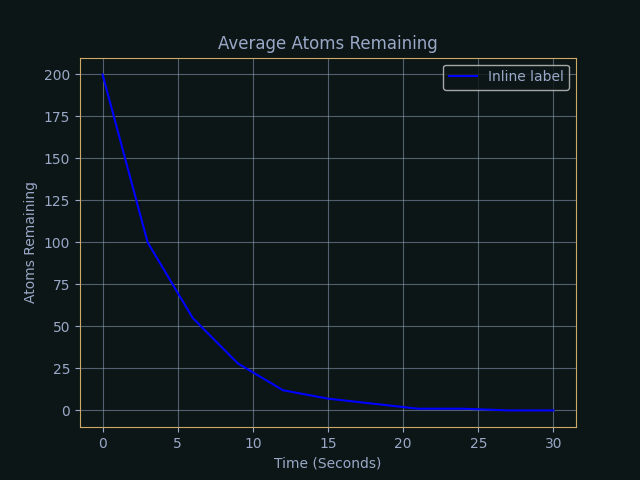
\includegraphics[width=\textwidth,height=\textheight,keepaspectratio]{latex-files/images/average-atoms-remaining.png}
  \label{fig:graph-for-the-average-atoms-remaining}
\end{center}

\newpage

\subsubsection{Conclusion}

Answer the following questions in complete sentences, and justify your responses.

\begin{enumerate}
  \item After how many time intervals (shakes) did one-half of your atoms
    (candies) decay? \\
    \bf{It took $1$ shake to get half of the atoms to decay.}

  \item What is the half-life of your substance? \\
    \bf{$3$ Seconds.}

  \item If the half-life model decayed perfectly, how many atoms would be
    remaining (not decayed) after 12 seconds? \\
    \bf{$12$ atoms will be left after $12$ seconds.}

  \item If you increased the initial number of atoms (candies) to 300, would the
    overall shape of the graph be altered? Explain your answer. \\
    \bf{Yes. The graph would start at a higher position, and it might endup
    taking a longer time for all of the atoms to decay. The reason why I said
    "it might" is because this is a random selection.}

  \item Go back to your data table and for each three-second interval, divide
    the number of candies decayed by the number previously remaining and
    multiply by 100. Show your work. \\
    \begin{align}
      \frac{100}{200} \times  100  &= 50         \\
      \frac{45}{100}  \times  100  &= 45         \\
      \frac{27}{55}   \times  100  &= 49.09      \\
      \frac{16}{28}   \times  100  &= 57.14      \\
      \frac{5}{12}    \times  100  &= 41.67      \\
      \frac{3}{7}     \times  100  &= 42.86      \\
      \frac{3}{4}     \times  100  &= 75         \\
      \frac{0}{1}     \times  100  &= 0          \\
      \frac{0}{0}     \times  100  &= 0          \\
    .\end{align}

  \item The above percentage calculation will help you compare the decay modeled
    in this experiment to the half-life decay of a radioactive element. Did this
    activity perfectly model the concept of half-life? If not, was it close? \\
    \bf{It didn't perfectly model the half-life decay of a radioactive element.
    But, it was very close.}

  \item Compare how well this activity modeled the half-life of a radioactive
    element. Did the activity model half-life better over the first 12 seconds
    (four decays) or during the last 12 seconds of the experiment? If you see
    any difference in the effectiveness of this half-life model over time, what
    do you think is the reason for it? \\
    \bf{The first $12$ seconds modeled the half-life the best.}
\end{enumerate}
